\newif\ifimagen\imagentrue
\documentclass[11pt]{article}
\usepackage[english,russian]{babel}\usepackage{fontspec}\usepackage{polyglossia}\usepackage{hyphenat}\usepackage{titlesec}\usepackage{ifthen}\usepackage{xkeyval}\usepackage[T1]{fontenc}\usepackage{graphicx}\usepackage[utf8]{inputenc}\usepackage{listings}\usepackage{cite}\usepackage{hevea}\newcommand{\Vspace}[1]{}
\newcommand{\Section}[1]{\Large\section{#1}\normalsize}
\newcommand{\SectionNo}[1]{\Large\section*{#1}\normalsize}
\newcommand{\SubSection}[1]{\large\subsection{#1}\normalsize}
\newcommand{\SubSectionNo}[1]{\large\subsection*{#1}\normalsize}
\newcommand{\SubSubSection}[1]{\large\subsubsection{#1}\normalsize}
\newcommand{\SubSubSectionNo}[1]{\large\subsubsection*{#1}\normalsize}
\newcommand{\parbox}[9]{{}\@br}
\newcommand{\includeimage}[3]{
\ifhevea
{
\imgsrc[style="margin-left: -20px;margin-botton: 30px; padding:20 20 20 20px;"]{\images/#1}\@br
Picture. {\bf #2}\@br\@br
}
\else
{
\begin{figure}[ht]
\centering
\includegraphics[scale=0.5]{#1}
\end{figure}}
\fi}
\newcommand{\ru}{}
\newcommand{\ti}{}
\newcommand{\verse}{\@open{div}{class="verse"}}
\newcommand{\endverse}{\@close{div}}
\newcommand{\siderules}{\@open{div}{class="siderules"}}
\newcommand{\endsiderules}{\@close{div}}
\newcommand{\tablefootnote}{}
\setcounter{secnumdepth}{0}
\let\oldmeta\@meta
  
\renewcommand{\@meta}{\begin{rawhtml}

  <meta name="Author" content="5HT">
  <meta charset="utf-8">
  <meta http-equiv="x-ua-compatible" content="ie=edge">
  <meta name="viewport" content="width=device-width, initial-scale=1">
  <link href="super-style.css" type="text/css" rel="stylesheet">
  <script src="super-code.js"></script>

  \end{rawhtml}}

\pagestyle{empty}
\thispagestyle{empty}
\begin{document}
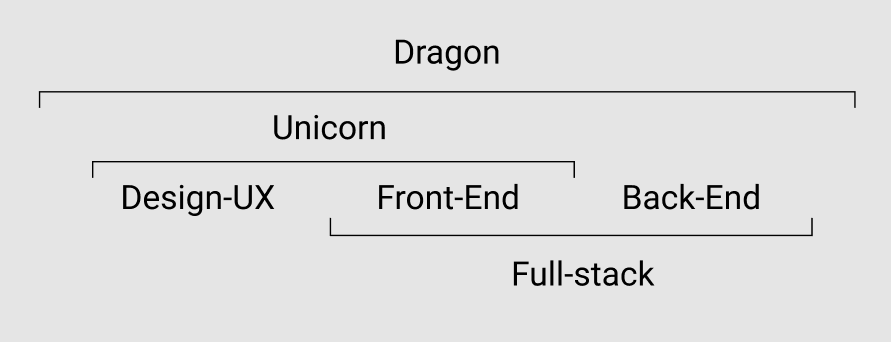
\includegraphics[scale=0.35]{./dragon.PNG}
\clearpage% page: 0
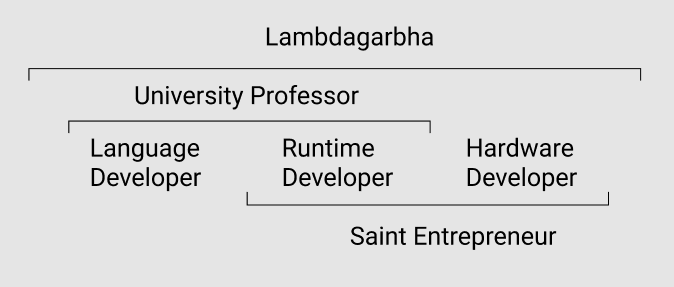
\includegraphics[scale=0.46]{./lambdagarbha.PNG}
\clearpage% page: 1
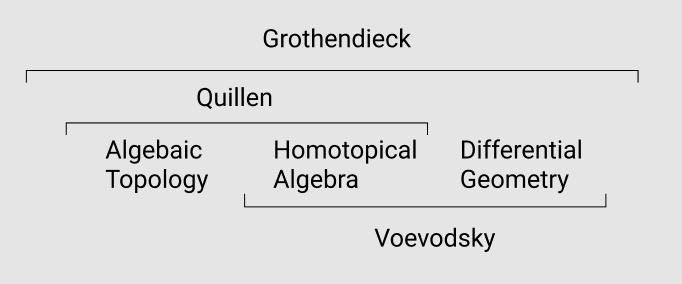
\includegraphics[scale=0.46]{./grothendieck.PNG}
\clearpage% page: 2
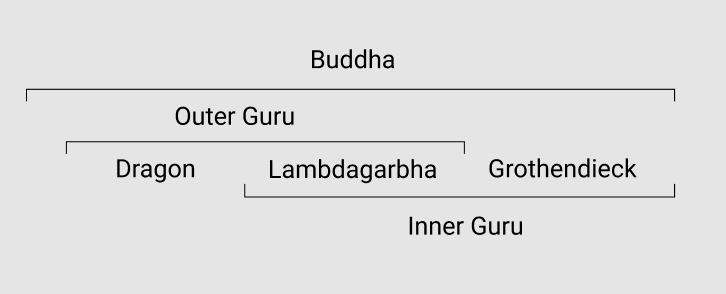
\includegraphics[scale=0.46]{./buddha.PNG}
\clearpage% page: 3
%Options: 
\end{document}
